%This work is licensed under the Creative Commons
%Attribution-ShareAlike 4.0 International License. To view a copy of
%this license, visit http://creativecommons.org/licenses/by-sa/4.0/ or
%send a letter to Creative Commons, PO Box 1866, Mountain View, CA
%94042, USA.

\documentclass[twoside,openright,titlepage,fleqn,
	headinclude,11pt,a4paper,BCOR5mm,footinclude
	]{scrbook}
%\documentclass[a4paper,11pt]{book}
\usepackage[utf8]{inputenc}
%\usepackage[latin1]{inputenc}
\usepackage{lmodern}
\usepackage{microtype}
\usepackage[T1]{fontenc}
%\usepackage[italian]{babel}
%\usepackage{graphicx}
\usepackage{subfiles}
\usepackage{listings}
%\usepackage{pgf}
\usepackage{xparse}
\usepackage{float}
\usepackage{color}
%\usepackage{xcolor}

%pacchetti del modello per la tesi
%--------------------------------------------------------------
\usepackage[square,numbers]{natbib} 
\usepackage[fleqn]{amsmath}  
\usepackage{dia-classicthesis-ldpkg} 
% Options for classicthesis.sty:
% tocaligned eulerchapternumbers drafting linedheaders 
% listsseparated subfig nochapters beramono eulermath parts 
% minionpro pdfspacing
\usepackage[eulerchapternumbers,subfig,beramono,eulermath,
	parts]{classicthesis}
%--------------------------------------------------------------
\usepackage{tikz}
\usetikzlibrary{shapes, chains, scopes, shadows, positioning, arrows,
  decorations.pathmorphing, calc, mindmap, petri}

\usepackage{cleveref}

%comandi per modello
%--------------------------------------------------------------
\newcommand{\myTitle}{B-Spline methods for designing smooth spatial
  path with obstacle avoidance\xspace}
% use the right myDegree option
\newcommand{\myDegree}{Master's degree in computer science\xspace}
\newcommand{\myName}{Stefano Martina\xspace}
\newcommand{\myMail}{stefano.martina@stud.unifi.it}
\newcommand{\myProf}{Alessandra Sestini\xspace}
%\newcommand{\myOtherProf}{Carlotta Giannelli\xspace}
\newcommand{\mySupervisor}{Carlotta Giannelli\xspace}
\newcommand{\myFaculty}{
	School of mathematical, physical and natural sciences\xspace}
\newcommand{\myDepartment}{
	Department of mathematics and computer science\xspace}
\newcommand{\myUni}{\protect{
	University of Florence}\xspace}
\newcommand{\myLocation}{Florence\xspace}
\newcommand{\myAcademicYear}{2015/2016\xspace}
\newcommand{\myYear}{2016\xspace}
\newcommand{\myVersion}{Version 0.1\xspace}
\newcommand{\mycopyright}{
  this work is licensed under a
  \href{http://creativecommons.org/licenses/by-sa/4.0/}{Creative
    Commons Attribution-ShareAlike 4.0 International License \includegraphics[width=1cm]{logo/logoCC.png}}\xspace}
\newlength{\abcd} % for ab..z string length calculation
% how all the floats will be aligned
\newcommand{\myfloatalign}{\centering} 
\setlength{\extrarowheight}{3pt} % increase table row height
\captionsetup{format=hang,font=small}
%--------------------------------------------------------------
% Layout setting
%--------------------------------------------------------------
\usepackage{geometry}
\geometry{
	a4paper,
	ignoremp,
	bindingoffset = 1cm, 
	textwidth     = 13.5cm,
	textheight    = 21.5cm,
	lmargin       = 3.5cm, % left margin
	tmargin       = 4cm    % top margin 
}
%--------------------------------------------------------------

%comando per impostazioni float di default
\makeatletter
\def\fps@figure{!htbp}
\def\fps@table{!htbp}
\def\fps@code{!htbp}
\makeatother

%cambia comportamento delle description
\renewcommand{\descriptionlabel}[1]{\hspace{2em}\hspace{\labelsep}\textbf{#1}}


%definisce un nuovo ambiente float per il codice
\newfloat{code}{!htbp}{}
\floatname{code}{Codice}

%comando per dimensioni testo
\newcommand{\dimg}{\tiny}
\newcommand{\codg}[1]{\dimg \unicocodet{#1}}
%  \lstinline[basicstyle=\dimg\ttfamily\bfseries,breaklines=true]|#1|


\newcommand{\dims}{\scriptsize}
\newcommand{\cods}[1]{\dims\unicocodet{#1}}
%  \lstinline[basicstyle=\dims\ttfamily\bfseries,breaklines=true]|#1|

\NewDocumentEnvironment{myfig}{mm}{
  \begin{figure}
    \begin{center}
    }{
    \end{center}
    \caption{#1}
    \label{#2}
  \end{figure}
}

%comando per inserire una immagine
\NewDocumentCommand{\image}{ommm}{
  \begin{figure}
    \begin{center}
      \begin{tikzpicture}
        \node [rectangle, rounded corners=2pt, inner sep = 0.3cm, drop shadow, draw=black!50, fill=white] {
          \IfNoValueTF{#1}
                      {\includegraphics[width=.9\textwidth]{#2}}
                      {\includegraphics[width=#1]{#2}}
        };
      \end{tikzpicture}
    \end{center}
    \caption{#3}
    \label{#4}
  \end{figure}
}

\NewDocumentCommand{\imageDouble}{ommmm}{
  \begin{figure}
    \begin{center}
      \begin{tikzpicture}
        \node [rectangle, rounded corners=2pt, inner sep = 0.3cm, drop shadow, draw=black!50, fill=white] {
          \IfNoValueTF{#1}
                      {\includegraphics[width=.42\textwidth]{#2}}
                      {\includegraphics[width=#1]{#2}}
        };
      \end{tikzpicture}
      \begin{tikzpicture}
        \node [rectangle, rounded corners=2pt, inner sep = 0.3cm, drop shadow, draw=black!50, fill=white] {
          \IfNoValueTF{#1}
                      {\includegraphics[width=.42\textwidth]{#3}}
                      {\includegraphics[width=#1]{#3}}
        };
      \end{tikzpicture}
    \end{center}
    \caption{#4}
    \label{#5}
  \end{figure}
}

\NewDocumentCommand{\imager}{ommm}{
  \begin{figure}
    \begin{center}
      \begin{tikzpicture}
        \node [rectangle, rounded corners=2pt, inner sep = 0.3cm, drop shadow, draw=black!50, fill=white, rotate = 90] {
          \IfNoValueTF{#1}
                      {\includegraphics[height=13cm]{#2}}
                      {\includegraphics[height=#1]{#2}}
        };
      \end{tikzpicture}
    \end{center}
    \caption{#3}
    \label{#4}
  \end{figure}
}

%comando per inserire un link
\newcommand{\link}[1]{\unicocode{#1}}


%comando per inserire un file
\newcommand{\file}[1]{\unicocode{#1}}

\newcommand{\bigO}{\ensuremath{\mathcal{O}}}

\def\transW{8mm}
\def\transH{2mm}

\tikzstyle{obstacle}=[fill=green, draw=black]
\tikzstyle{convexHull}=[fill=blue!30]
\tikzstyle{convexHullBord}=[color=black, dash pattern=on 3pt off 3pt]
\tikzstyle{controlPoly}=[color=black, line width=0.25mm]
\tikzstyle{controlPolyTract}=[color=black, line width=0.25mm, dash pattern=on 3pt off 3pt]
\tikzstyle{controlPolyTractHigh}=[color=red, line width=0.25mm, dash pattern=on 3pt off 3pt]
\tikzstyle{obstacleTract}=[draw=black, line width=0.25mm, dash pattern=on 3pt off 3pt]
\tikzstyle{spline}=[color=red, line width=0.5mm]
\tikzstyle{controlVert}=[color=green, draw=black]
\tikzstyle{controlVertHigh}=[color=red, draw=black]
\tikzstyle{obstaclePoint}=[color=red, draw=black]
\tikzstyle{site}=[color=blue, draw=black]
\tikzstyle{siteHigh}=[color=red, draw=black]
\tikzstyle{textArrow}=[draw=red, line width=0.5mm, ->]

\colorlet{mmcb}{black!70}
\colorlet{mmc1}{red!80}
\colorlet{mmc2}{blue!80}
\colorlet{c1}{green!20}
\colorlet{c2}{blue!10}
\colorlet{c3}{yellow!10}
\colorlet{c4}{red!10}
\colorlet{drawColor}{black!80}
\colorlet{commentColor}{green!70!black!90}
\colorlet{codeBgColor}{yellow!50}
\colorlet{bashBgColor}{green!50}

\tikzset{onslide/.code args={<#1>#2}{%
  \only<#1>{\pgfkeysalso{#2}} % \pgfkeysalso doesn't change the path
}}
\tikzset{temporal/.code args={<#1>#2#3#4}{%
  \temporal<#1>{\pgfkeysalso{#2}}{\pgfkeysalso{#3}}{\pgfkeysalso{#4}} % \pgfkeysalso doesn't change the path
}}

\tikzstyle{alertStar}=[circle, decorate, decoration={zigzag,segment length=3.12mm,amplitude=1mm}, align=center, drop shadow, draw=drawColor, fill=white]
\tikzstyle{oval}=[ellipse, align=center, drop shadow, draw=drawColor, fill=white]
\tikzstyle{rect}=[rectangle, rounded corners=2pt, align=center, drop
shadow, draw=drawColor, fill=white]
\tikzstyle{arrow}=[->, very thick, >=stealth', draw=black!80]
\tikzstyle{myMindmap}=[mindmap,
every node/.style={concept, minimum size=5mm, text width=5mm}, 
% every child/.style={level distance=10mm, concept color=mmcb}
level 1/.append style={level distance=10mm,sibling angle=45},
level 2/.append style={level distance=10mm,sibling angle=45},
level 3/.append style={level distance=10mm,sibling angle=45}
]
\tikzstyle{myPlace} = [place, very thick, draw=drawColor, fill=white, drop shadow]
\tikzstyle{transExpH} = [transition, very thick, draw=drawColor, fill=white, drop
shadow, minimum width=\transW, minimum height=\transH]
\tikzstyle{transExpV} = [transition, very thick, draw=drawColor, fill=white, drop
shadow, minimum width=\transH, minimum height=\transW]
\tikzstyle{transDetH} = [transition, very thick, draw=drawColor, fill=black, drop shadow, minimum width=\transW, minimum height=\transH]
\tikzstyle{transDetV} = [transition, very thick, draw=drawColor, fill=black, drop shadow, minimum width=\transH, minimum height=\transW]
\tikzstyle{pre}=[<-, very thick, >=stealth', draw=drawColor]
\tikzstyle{preN}=[<-, very thick, >=o, draw=drawColor]
\tikzstyle{post}=[->, very thick, >=stealth', draw=drawColor]
\tikzstyle{highlight}=[draw=red]
\lstdefinestyle{customPython}{
   language=Python,
   % basicstyle=\small\ttfamily\bfseries,
   basicstyle=\tiny\ttfamily,
   keywordstyle=\color{blue}\ttfamily,
   stringstyle=\color{red}\ttfamily,
   commentstyle=\color{green}\ttfamily,
   morecomment=[l][\color{magenta}]{\#},
   % breaklines=false,
   breaklines=true, breakatwhitespace=true,
   postbreak=\raisebox{0ex}[0ex][0ex]{\ensuremath{\color{red}\hookrightarrow\space}},
   frameround=fttt,
   frame=trBL,
   backgroundcolor=\color{yellow!20},
   numbers=left,
   stepnumber=1,    
   firstnumber=1,
   numberfirstline=true,
   numberstyle=\tiny\color{black!50},
   xleftmargin=1.75em,
   framexleftmargin=2.1em,
   % rulesepcolor=\color{gray},
   rulecolor=\color{black}
   % linewidth=8cm,
}

\lstdefinestyle{customInlinePython}{
   language=Python,
   % basicstyle=\small\ttfamily\bfseries,
   basicstyle=\ttfamily,
   keywordstyle=\color{blue}\ttfamily,
   stringstyle=\color{red}\ttfamily,
   commentstyle=\color{green}\ttfamily,
   morecomment=[l][\color{magenta}]{\#}
}

\lstnewenvironment{pblock}[1][]
{
  \lstset{
    style=customPython,
    #1
  }
}{}

\newcommand{\pfile}[2][]{
  \lstinputlisting[style=customPython, title={\texttt{\detokenize{#2}}}, #1]{#2}
}

\newcommand{\pp}[2][]{\lstinline[style=customInlinePython,#1]`#2`}
  %\colorbox{codeBgColor}{
  %  \lstinline[style=customPython,#1]`#2`
  %}
%}

\graphicspath{{img/}}
\lstset{inputpath=src/}

%% \definecolor{links}{HTML}{2A1B81}
%% \hypersetup{colorlinks,linkcolor=links,urlcolor=links}

%% \definecolor{links}{HTML}{2A1B81}
%% \hypersetup{colorlinks,linkcolor=,urlcolor=links}

\newcommand{\me}{\ensuremath{\mathrm{e}}}
\newcommand{\md}{\ensuremath{\mathrm{d}}}
\newcommand{\tc}{\ensuremath{\mathrm{t.c.:}\quad}}
\newcommand{\expected}[1]{\ensuremath{\mathrm{\textbf{E}}\left[#1\right]}}
\newcommand{\variance}[1]{\ensuremath{\mathrm{\textbf{Var}}\left(#1\right)}}
\newcommand{\prob}[1]{\ensuremath{\mathrm{\textbf{P}}\left(#1\right)}}
%\newcommand{\max}[1]{\ensuremath{\mathrm{max}\left(#1\right)}}
\newcommand{\abs}[1]{\ensuremath{\left|#1\right|}}
\newcommand{\mR}{\ensuremath{\mathbb{R}}}
\newcommand{\mN}{\ensuremath{\mathbb{N}}}


%%% Local Variables:
%%% mode: latex
%%% TeX-master: "dissertation"
%%% End:



\begin{document}

\title[Trijkstra]{\textbf{Trijkstra}}
\date[4 December 2015]{\flushright 4 December 2015}
\subtitle{A Dijkstra algorithm application to path planning}
\institute[Uni. Firenze]{
  \includegraphics[width=5cm]{img/logoUnifiName.eps}
}

\author[Martina Stefano]{
  \begin{center}
    \begin{tabular}{lr}
      Stefano \textsc{Martina}\\
      \href{mailto:stefano.martina@stud.unifi.it}{stefano.martina@stud.unifi.it}\\
    \end{tabular}
  \end{center}
}

\titlegraphic{
  \vspace{-0.5cm}
  \tiny
  \href{http://creativecommons.org/licenses/by-sa/4.0/}{\includegraphics[width=1cm]{img/logoCC.png}}
  This work is licensed under a
  \href{http://creativecommons.org/licenses/by-sa/4.0/}{Creative
    Commons Attribution-ShareAlike 4.0 International License}.
}

\newacro{VD}{Voronoi Diagram}

\acrodefplural{VD}[VDs]{Voronoi Diagrams}

\begin{frame}[plain]
  \titlepage
\end{frame}

\section{Prerequisites}

\begin{frame}
  \frametitle{Voronoi diagrams}
  \begin{description}
  \item[Input:] A set of points in plane (or space) called
    \alert{sites}
  \item[Output:]<2-> A partition of the plane (or space) such that each
    point of a \alert{region} is nearer to a certain site respect to
    the others
  \end{description}
  \begin{columns}
    \begin{column}{0.5\textwidth}
      \begin{center}
        \includegraphics[width=\textwidth]{img/voroSites.eps}
      \end{center}
    \end{column}
    \begin{column}{0.5\textwidth}
      \begin{center}
        \includegraphics[width=\textwidth]<2->{img/voronoi.eps}
      \end{center}
    \end{column}
  \end{columns}
\end{frame}

\begin{frame}
  \frametitle{B-spline}
  \begin{center}
    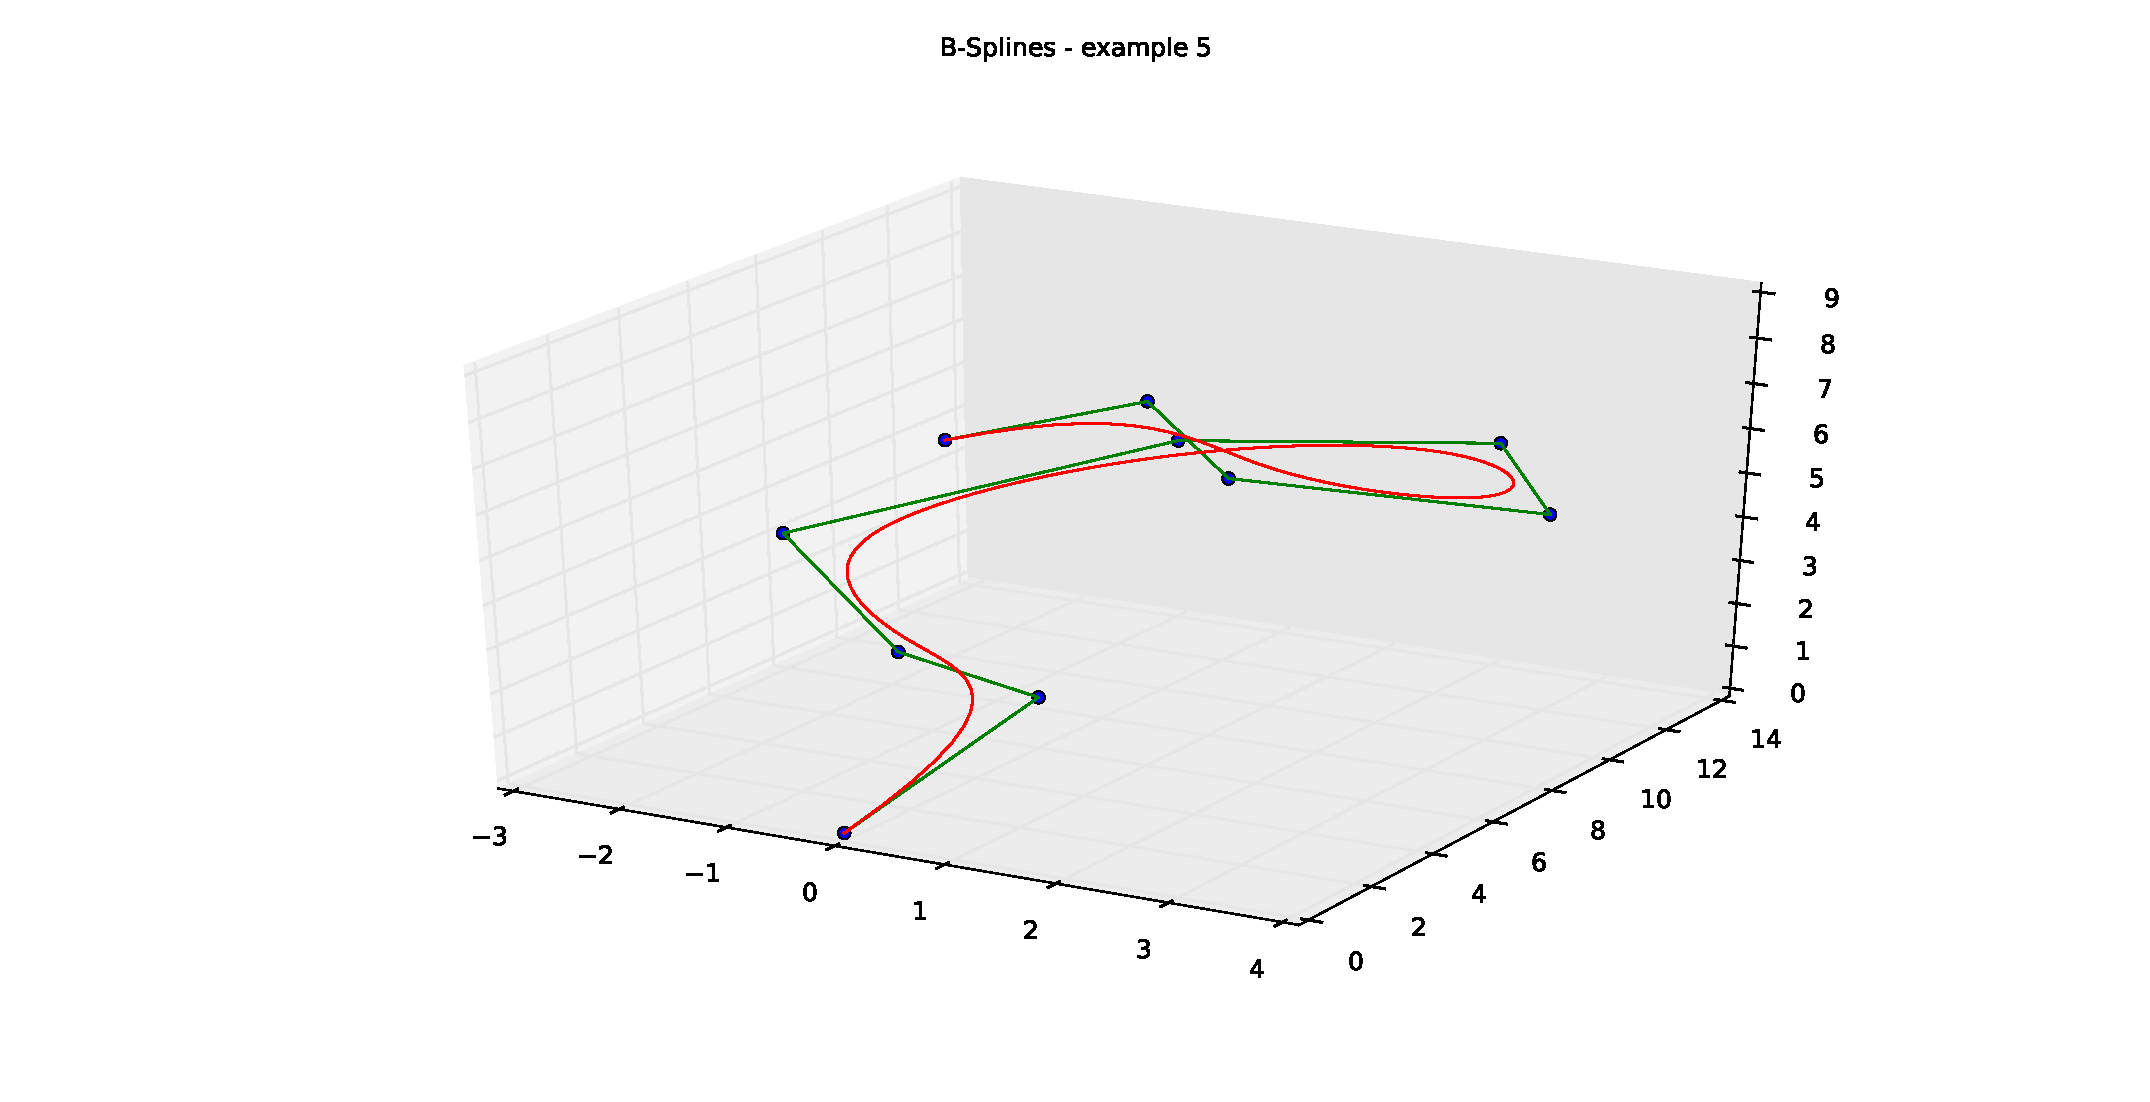
\includegraphics[width=0.9\textwidth, trim=110 30 50 50, clip]{img/bspline.eps}
  \end{center}
  \pause
  \begin{itemize}
  \item \alert{parametric} curves\pause
  \item follow the shape of a \alert{control poligon}\pause
  \item can interpolate the
    \alert{extremes} of the control polygon
  \end{itemize}
\end{frame}

\begin{frame}[fragile]
  \frametitle{Dijkstra algorithm}
  \begin{pblock}
def dijkstra(graph, start, end):
  path = []
  Q = priorityQueue.PQueue()
  dist = {}
  prev = {}
  for node in graph.nodes(): #populate the queue
    if node != start:
      dist[node] = inf
      Q.add(node, inf)
    else:
      dist[node] = 0
      Q.add(node, 0)
  while True:  #main loop
    u = Q.pop() #take nearest node and remove from queue
    if u == end or dist[u] == inf: #finished (good or bad)
      break
    #all neighbors still in queue
    for v in Q.filterGet(lambda node: node in graph.neighbors(u)):
      tmpDist = dist[u] + graph[u][v]['weight']
      if tmpDist < dist[v]: #if distance shorter update values
        dist[v] = tmpDist
        prev[v] = u
        Q.add(v, tmpDist) #update distance also in queue
  u = end
  while u in prev:  #backward recreation of path
      u = prev[u]
      path[:0] = [u]
  if path:
      path[len(path):] = [end]
      path[:0] = [start]
  return path
  \end{pblock}  
\end{frame}

\section{Background}

\begin{frame}
  \frametitle{Background}
  \begin{block}{Main problem}
    \alert{Path planning} from a \alert{start} point to an \alert{end}
    point in 3D space with obstacles using \alert{Voronoi} diagrams.
  \end{block}\pause
  \begin{enumerate}
  \item Distribute \alert{points} in the surfaces of obstacles
    \begin{itemize}
    \item and optionally in the surface of bounding box\pause
    \end{itemize}
  \item Build \alert{Voronoi} diagram using those points as
    source\pause
  \item Transform the Voronoi diagram in a \alert{graph}
    \begin{itemize}
    \item cells \alert{vertexes} as \alert{nodes}
    \item cells \alert{edges} as \alert{arcs} (infinite edges
      ignored)\pause
    \end{itemize}
  \item \alert{Prune} the arcs that crosses an obstacle's
    surface\pause
  \item Attach the \alert{start} and \alert{end} points to the
    graph as nodes\pause
  \item Calculate the shortest path from start node to end node using
    \alert{Dijkstra}'s algorithm.
  \end{enumerate}
\end{frame}

\begin{frame}
  \frametitle{Example}
  \begin{center}
    \includegraphics[width=0.75\textwidth, trim=110 30 50 50, clip]<1>{img/screen1.eps}
    \includegraphics[width=0.75\textwidth, trim=110 30 50 50, clip]<2>{img/screen2.eps}
    \includegraphics[width=0.75\textwidth, trim=110 30 50 50, clip]<3>{img/screen3.eps}
    \includegraphics[width=0.75\textwidth, trim=110 30 50 50, clip]<4>{img/screen4.eps}
    \includegraphics[width=0.75\textwidth, trim=110 30 50 50, clip]<5>{img/screen5.eps}
  \end{center}
\end{frame}

\section{Implementation}

\begin{frame}
  \frametitle{Improvement}
  \begin{block}{Idea}
    Make a \alert{smoother} curve instead of finding the polygonal chain
    of the shortest path in the structure
  \end{block}
  \pause
  \begin{itemize}
  \item we can use a \alert{B-Spline} that \pause
    \begin{itemize}
    \item \alert{interpolate} the start and end vertexes\pause
    \item use the shortest path found with
      Dijkstra as \alert{control polygon}
    \end{itemize}
  \end{itemize}
\end{frame}

\begin{frame}
  \frametitle{Problem}  
  \begin{itemize}
  \item The \alert{control polygon} is free from obstacles by
    construction\pause
    \begin{itemize}
    \item (the graph is pruned of the arcs that cross an obstacle's surface)\pause
    \end{itemize}
  \item But the \alert{curve} is not guaranteed to be free from obstacles\pause
  \end{itemize}
  \begin{center}
    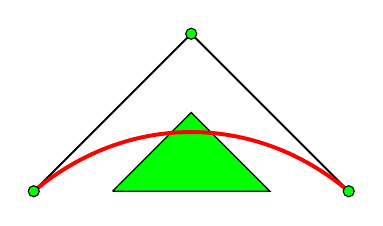
\begin{tikzpicture}
      \path[obstacle] (1,0) -- (2,1) -- (3,0) -- (1,0);
      \draw[controlPoly] (0,0) -- (2,2) -- (4,0);
      \draw[spline] (0,0) to [bend left=40] (4,0);

      \filldraw[controlVert] (0,0) circle (2pt);
      \filldraw[controlVert] (2,2) circle (2pt);
      \filldraw[controlVert] (4,0) circle (2pt);
    \end{tikzpicture}
  \end{center}
\end{frame}

\begin{frame}
  \frametitle{Solution}
  \begin{itemize}
  \item A \alert{B-Spline} of order \alert{$n$} is contained
    inside the union of \alert{convex hulls} composed of consecutive
    \alert{$n$} vertexes of control polygon\pause
  \end{itemize}
  \begin{center}
    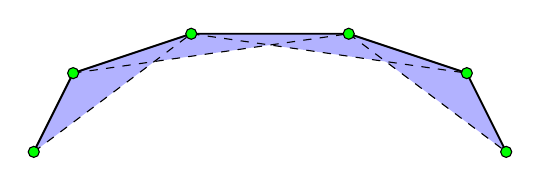
\begin{tikzpicture}
      \coordinate (a) at (0,0);
      \coordinate (b) at (0.5,1);
      \coordinate (c) at (2,1.5);
      \coordinate (d) at (4,1.5);
      \coordinate (e) at (5.5,1);
      \coordinate (f) at (6,0);

      \path[convexHull] (a) -- (b) -- (c) -- (a);
      \path[convexHull] (b) -- (c) -- (d) -- (b);
      \path[convexHull] (c) -- (d) -- (e) -- (c);
      \path[convexHull] (d) -- (e) -- (f) -- (d);

      \draw[convexHullBord] (a) -- (c);
      \draw[convexHullBord] (b) -- (d);
      \draw[convexHullBord] (c) -- (e);
      \draw[convexHullBord] (d) -- (f);

      \draw[controlPoly] (a) -- (b) -- (c) -- (d) -- (e) -- (f);
      \foreach \p in {a,b,c,d,e,f}
      \filldraw[controlVert] (\p) circle (2pt);
    \end{tikzpicture}
  \end{center}
  \pause
  \begin{block}{Idea}
    \begin{itemize}
    \item we can use a \alert{quadratic} B-Spline (grade 2, order 3) to smooth the
      path\pause
    \item and \alert{keep} triangles formed by three
      consecutive points
      \alert{free} from obstacles
    \end{itemize}
  \end{block}
\end{frame}

\begin{frame}
  \frametitle{Implementation}
  \begin{tikzpicture}[remember picture,overlay]
    \path[textArrow]<11-> ([xshift=-5.5mm,yshift=1mm]tloop2.west) to [out=180, in=180,distance=7mm] ([xshift=-5.5mm,yshift=1mm]tloop1.west);
  \end{tikzpicture}
  A variation of \alert{Dijkstra} algorithm is developed where:\pause
  \begin{enumerate}
  \item create an ordered \alert{triple} for each three consecutive nodes in the graph\pause
  \item check if the \alert{triangle} corresponding to each triple
    \alert{intersect} an obstacle\pause
  \item populate the \alert{priority queue} with obstacle free
    \alert{triples}\pause
    \begin{itemize}
    \item the initial weight is \alert{$0$} for triples where the
      \alert{first} node is the \alert{start} node\pause
    \item is \alert{$\infty$} otherwise\pause
    \end{itemize}
  \item\label{item:trijkstraLoop}\tikz[remember picture] \node[coordinate] (tloop1) {};pop the triple with \alert{lowest} weight from the priority
    queue\pause
  \item update the weight and pointer to previous of all \alert{neighbouring} triples\pause
    \begin{itemize}
    \item a triple $B$ is \alert{subsequent} to a triple $A$ if
      \alert{$(A[2]=B[1])\land (A[3]=B[2])$}\pause
    \item the \alert{weight} of a neighbour is \alert{$W(B)=W(A)+dist(A[1],A[2])$}\pause
    \end{itemize}
  \item\tikz[remember picture] \node[coordinate] (tloop2) {};repeat from point~\ref{item:trijkstraLoop} until popped a
    special \alert{ending} triple or a triple with weight
    \alert{$\infty$}\pause
  \item the shortest \alert{path} (with free triangular convex hull)
    can be 
    obtained following the \alert{previous} pointer from the
    \alert{ending} triple,
    and \alert{deconstructing} the triples
  \end{enumerate}
\end{frame}

\section{Code}

\begin{frame}[fragile]
  \frametitle{Declarations \& Triples creation}
  \begin{pblock}
def _trijkstra(self, startA, endA):
  start = tuple(startA)
  end = tuple(endA)
  endTriplet = (end,end,end) #special triplet for termination
  inf = float("inf")
  path = []
  Q = priorityQueue.PQueue()
  dist = {}
  prev = {}
  hits = []
  \end{pblock}
  \begin{pblock}
  for node0 in self._graph.nodes():
    for node1 in self._graph.neighbors(node0):
      for node2 in filter(lambda node: node!=node0, self._graph.neighbors(node1)):
        triplet = (node0,node1,node2)
        if not triplet[::-1] in hits:
          if not self._triangleIntersectPolyhedrons(np.array(node0), np.array(node1), np.array(node2)):
            if node0 != start:
              dist[triplet] = inf
              Q.add(triplet, inf)
            else:
              dist[triplet] = 0
              Q.add(triplet, 0)
          else:
            hits[:0] = [triplet]

  dist[endTriplet] = inf
  Q.add(endTriplet, inf)
  \end{pblock}
\end{frame}

\begin{frame}[fragile]
  \frametitle{Main loop}
  \begin{pblock}
while True:
  u = Q.pop()

  if u == endTriplet or dist[u] == inf:
    break

  for v in Q.filterGet(lambda tri: u[1] == tri[0] and u[2] == tri[1]):
    tmpDist = dist[u] + self._graph[u[0]][u[1]]['weight']
    if tmpDist < dist[v]:
      dist[v] = tmpDist
      prev[v] = u
      Q.add(v, tmpDist)

  if u[2] == end:
    tmpDist = dist[u] + self._graph[u[0]][u[1]]['weight'] + self._graph[u[1]][u[2]]['weight']
    if tmpDist < dist[endTriplet]:
      dist[endTriplet] = tmpDist
      prev[endTriplet] = u
      Q.add(v, tmpDist)
  \end{pblock}
\end{frame}

\begin{frame}[fragile]
  \frametitle{Path creation}
  \begin{pblock}
u = endTriplet
while u in prev:
  u = prev[u]
  path[:0] = [u[1]]

if path:
  path[len(path):] = [end]
  path[:0] = [start]

return np.array(path)
  \end{pblock}\pause
  \begin{block}{After}
    we can use the returned \alert{path} as a \alert{control polygon}
    for a quadratic
    B-Spline without problems, and construct a smoother path.
  \end{block}
\end{frame}

\section{Conclusion}

\begin{frame}
  \frametitle{Previous example}
  \begin{center}
    \includegraphics[width=0.75\textwidth, trim=110 30 50 50, clip]{img/screenFinal.eps}
  \end{center}
\end{frame}

\begin{frame}
  \frametitle{Clearer example}
  \begin{center}
    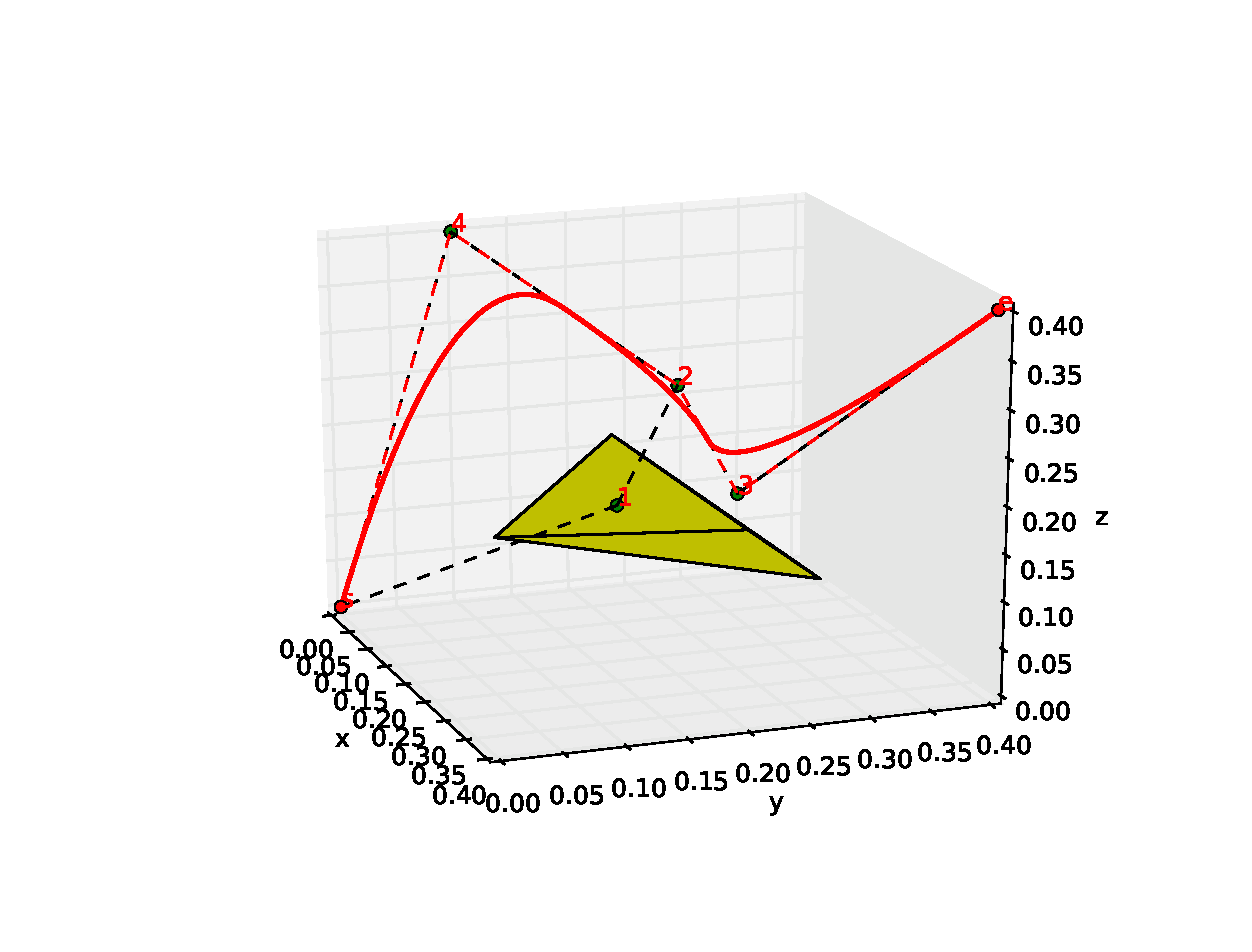
\includegraphics[width=0.75\textwidth, trim=110 30 50 50, clip]{img/screenFinal2.eps}
  \end{center}
\end{frame}

\begin{frame}
  \frametitle{Complexity considerations}
  The algorithm is analogous to classical \alert{Dijkstra} applied to a
  \alert{transformed} graph where:\pause
  \begin{itemize}
  \item the original graph is \alert{not} directed and weighted\pause
  \item the transformed graph is \alert{directed} and weighted,
    and\pause
    \begin{itemize}
    \item if \alert{$A$} and \alert{$B$} are \alert{neighbouring} and
      \alert{$B$} and \alert{$C$} are \alert{neighbouring}, in the original graph\pause
    \item we have two nodes \alert{$(A,B,C)$} and
      \alert{$(C,B,A)$} in the transformed graph\pause
    \item a node \alert{$(A_1,B_1,C_1)$} is a predecessor of
      \alert{$(A_2,B_2,C_2)$} in the transformed graph if
      \alert{$B_1=A_2$} and \alert{$C_1=B_2$} in the original graph\pause
    \item and the weight of the arc is the weight of the original from
      \alert{$A_1$} to \alert{$B_1(=A_2)$}
    \end{itemize}
  \end{itemize}
\end{frame}

% \begin{frame}
%   \frametitle{Time complexity (rough worst case scenario)}
%   \begin{itemize}
%   \item If the original graph is a \alert{clique}\pause
%   \item cost of \alert{Dijkstra}: $\bigO(|E_{mod}|+|V_{mod}|\log |V_{mod}|)=$\alert{$\bigO(|V_{mod}|^2)$}\pause
%   \item where the number $|V_{mod}|$ of nodes is the
%     number of 3-permutation of the original nodes: $|V_{orig}|\cdot
%     (|V_{orig}|-1)\cdot(|V_{orig}|-2)=$\alert{$\bigO(|V_{orig}|^3)$}\pause
%   \item plus a negligible \alert{$\bigO(|V_{orig}|^3)$} for the triples
%     creation\pause
%   \end{itemize}
%   \begin{block}{In total}
%     \alert{$$\bigO(|V_{orig}|^6)$$}
%   \end{block}
%   \pause
%   \begin{block}{But}
%     \begin{itemize}
%     \item The original graph is not a \alert{clique}, is a
%       lattice\pause
%     \item Maybe too pessimistic assuming
%       $|E_{mod}|=\bigO(|V_{mod}|^2)$\pause
%     \item Still need to study deeper the complexity
%     \end{itemize}
%   \end{block}
% \end{frame}

\begin{frame}
  \frametitle{Time complexity (For original graph creation)}
  \begin{itemize}
  \item \alert{Fortune} algorithm run in \alert{$\bigO(n\log n)$}\pause
  \item if we have $n$ input sites we get \alert{$\bigO(n)$} vertexes
    of Voronoi areas\pause
  \item if we assume obstacles with a maximum area\pause
    \begin{itemize}
    \item \alert{$\bigO(|Ob|)$} input sites\pause
    \end{itemize}
  \end{itemize}
  \begin{block}{Total}
    \begin{itemize}
    \item \alert{$\bigO(|Ob|\log |Ob|)$}\pause
    \item The number of vertexes of the graph is \alert{$|V_{orig}|=\bigO(|Ob|)$}
    \end{itemize}
  \end{block}
\end{frame}

\begin{frame}
  \frametitle{Time complexity (For modified graph creation)}
  \begin{itemize}
  \item Suppose that the graph has a maximum degree \alert{$k$}\pause
    \begin{itemize}
    \item each node has maximum $k$ \alert{neighbours}\pause
    \end{itemize}
  \item Cost for triples \alert{creation}: $|V_{orig}|\cdot k\cdot
    (k-1)=$\alert{$\bigO(k^2|V_{orig}|)$}\pause
    \begin{itemize}
    \item plus for each triple and each obstacle solve a $4\times 4$
      linear system for the collision check\pause
    \item cost for creation and check: \alert{$\bigO(|Ob|k^2|V_{orig}|)$}\pause
    \end{itemize}
  \end{itemize}
  \begin{block}{Total}
    \alert{$\bigO(|Ob|^2k^2)$}
  \end{block}
\end{frame}

\begin{frame}
  \frametitle{Time complexity (Routing in modified graph)}
  \begin{itemize}
  \item
    \begin{minipage}[t]{0.8\linewidth}
      Each \alert{node} is the \alert{central} point of $2\cdot
      \binom{k}{2}=k\cdot(k-1)$ triples
    \end{minipage}\hfill
    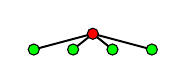
\begin{tikzpicture}
      \coordinate (r) at (0.75,0.2);
      \coordinate (a) at (0,0);
      \coordinate (b) at (0.5,0);
      \coordinate (c) at (1,0);
      \coordinate (d) at (1.5,0);
      \draw[controlPoly] (a) -- (r) -- (b);
      \draw[controlPoly] (c) -- (r) -- (d);
      
      \filldraw[controlVert,fill=red] (r) circle (2pt);
      \foreach \p in {a,b,c,d}
      \filldraw[controlVert] (\p) circle (2pt);
    \end{tikzpicture}\pause

    \begin{itemize}
    \item $|V_{mod}|=|V_{orig}|\cdot k\cdot(k-1)=$\alert{$\bigO(k^2|V_{orig}|)$}\pause
    \end{itemize}
  \item 
    \begin{minipage}[t]{0.8\linewidth}
      Each \alert{triple} is a \alert{predecessor} of $k-1$ triples
    \end{minipage}\hfill
    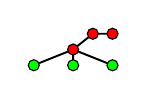
\begin{tikzpicture}
      \coordinate (r) at (0.5,0.2);
      \coordinate (a) at (0,0);
      \coordinate (b) at (0.5,0);
      \coordinate (c) at (1,0);
      \coordinate (s) at (0.75,0.4);
      \coordinate (t) at (1,0.4);
      \draw[controlPoly] (a) -- (r) -- (b);
      \draw[controlPoly] (c) -- (r);
      \draw[controlPoly] (r) -- (s) -- (t);
      
      \foreach \p in {r,s,t}
      \filldraw[controlVert,fill=red] (\p) circle (2pt);
      \foreach \p in {a,b,c}
      \filldraw[controlVert] (\p) circle (2pt);
    \end{tikzpicture}\pause

    \begin{itemize}
    \item $|E_{mod}|=|V_{mod}|\cdot (k-1)=\bigO(k|V_{mod}|)=$\alert{$\bigO(k^3|V_{orig}|)$}\pause
    \end{itemize}
  \item Cost of \alert{Dijkstra}: $\bigO(|E_{mod}|+|V_{mod}|\log
    |V_{mod}|)=$\alert{$\bigO(k^3|V_{orig}|+ k^2|V_{orig}|\log(k|V_{orig}|))$}
  \end{itemize}
\end{frame}

\begin{frame}
  \frametitle{Special cases}
  \begin{itemize}
  \item $\bigO(k^3|V_{orig}|+ k^2|V_{orig}|\log(k|V_{orig}|))$\pause
  \end{itemize}

  \begin{block}{If $k$ is constant (don't grow with $|V_{orig}|$)}
    \begin{itemize}
    \item Total cost: \alert{$\bigO(|V_{orig}|\log|V_{orig}|)$}\pause
    \item same cost of Dijkstra in a lattice\pause
    \end{itemize}
  \end{block}
  \begin{block}{If the graph is a clique}
    \begin{itemize}
    \item $k=|V_{orig}|-1$\pause
    \item Total cost: \alert{$\bigO(|V_{orig}|^4)$}
    \end{itemize}
  \end{block}
\end{frame}

\begin{frame}
  \frametitle{Overall}
  \begin{block}{Total (if obstacle area is not a function of the
      number of obstacles)}
    \alert{$\bigO(k^2|Ob|^2+k^3|Ob|)$}\pause
  \end{block}
  \begin{itemize}
  \item The predominant factor is for checking the triples
    collisions with obstacles\pause
    \begin{itemize}
    \item if $k$ is constant \alert{$\bigO(|Ob|^2)$}\pause
    \end{itemize}
  \item But if we focus only on routing (i.e. we construct the graph
    only once)\pause
    \begin{itemize}
    \item if $k$ is constant \alert{$\bigO(|Ob|\log|Ob|)$}
    \end{itemize}
  \end{itemize}
\end{frame}

\begin{frame}
  \begin{center}
	\textbf{\calligra\Huge The End.}\\
  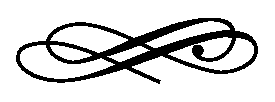
\includegraphics[width=5cm]{img/ornament.eps}\\[1cm]
	\pause
	{\huge\calligra Questions?\pause{} Thank you!}
  \end{center}
\end{frame}
\end{document}